\documentclass[a4paper,12pt]{article}
%%%%%%%%%%%%%%%%%%%%%%%%%%%%%%%%%%%%%%%%%%%%%%%%%%%%%%%%%%%%%%%%%%%%%%%%%%%%%%%%%%%%%%%%%%%%%%%%%%%%%%%%%%%%%%%%%%%%%%%%%%%%%%%%%%%%%%%%%%%%%%%%%%%%%%%%%%%%%%%%%%%%%%%%%%%%%%%%%%%%%%%%%%%%%%%%%%%%%%%%%%%%%%%%%%%%%%%%%%%%%%%%%%%%%%%%%%%%%%%%%%%%%%%%%%%%
\usepackage{eurosym}
\usepackage{vmargin}
\usepackage{amsmath}
\usepackage{graphics}
\usepackage{epsfig}
\usepackage{subfigure}
\usepackage{fancyhdr}
%\usepackage{listings}
\usepackage{framed}
\usepackage{graphicx}

\setcounter{MaxMatrixCols}{10}
%TCIDATA{OutputFilter=LATEX.DLL}
%TCIDATA{Version=5.00.0.2570}
%TCIDATA{<META NAME="SaveForMode" CONTENT="1">}
%TCIDATA{LastRevised=Wednesday, February 23, 2011 13:24:34}
%TCIDATA{<META NAME="GraphicsSave" CONTENT="32">}
%TCIDATA{Language=American English}

\pagestyle{fancy}
\setmarginsrb{20mm}{0mm}{20mm}{25mm}{12mm}{11mm}{0mm}{11mm}
\lhead{Dublin \texttt{R}} \rhead{10 April 2013}
\chead{Introduction to \texttt{R} (Module A)}
%\input{tcilatex}

\begin{document}
\newpage
\subsection{Exercise Data Set}
The exercise data set comes from a survey of home owners
conducted by an electricity company about an offer of roof solar panels with a 50\% subsidy
from the state government as part of the state’s environmental policy. The variables involve
household income measured in units of a thousand dollars, age, monthly mortgage, size of
family household, and as the dependent variable, whether the householder would take or decline the offer.
The purpose of the exercise is to conduct a logistic regression to determine whether family
size and monthly mortgage will predict taking or declining the offer.

For the first demonstration, we will use `family size’ and
`mortgage’ only. For the options, select Classification Plots, Hosmer-Lemeshow Goodness
Of Fit, Casewise Listing Of Residuals and select Outliers Outside 2sd. Retain default
entries for probability of stepwise, classification cutoff and maximum iterations.

\begin{figure}[h!]
	\begin{center}
		% Requires \usepackage{graphicx}
		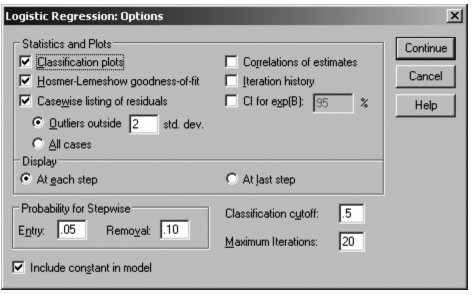
\includegraphics[scale=0.8]{images/Logistic10}\\
		\caption{Selected Options for Exercises}
	\end{center}
\end{figure}

We are not using any categorical variables this time. If there are categorical variables, use the \textbf{\textit{categorical}} option. For most situations, choose the ‘indicator’ coding scheme (it is the
default).
\subsection{HSB2 Example}
The hsb2 dataset is taken from a national survey of high school seniors. Two hundred observation were randomly sampled from the High School and Beyond survey. Descriptive statistics and exploratory data analysis are shown below.
Because we do not have a suitable dichotomous variable to use as our dependent variable, we will create one (which we will call honcomp, for honors composition) based on the continuous variable write.  We do not advocate making dichotomous variables out of continuous variables; rather, we do this here only for purposes of this illustration.


Here is the list of variables in the file.
\begin{verbatim}

  obs:           200    highschool and beyond (200 cases)
 vars:            12    28 Feb 2005 09:25
-----------------------------------------------------------------------------
              variable
variable name   type   about the variable
-----------------------------------------------------------------------------
id              scale  student id
female        nominal  (0/1)
race          nominal  ethnicity (1=hispanic 2=asian 3=african-amer 4=white)
ses           ordinal  (1=low 2=middle 3=high)
schtyp        nominal  type of school (1=public 2=private)
prog          nominal  type of program (1=general 2=academic 3=vocational)
read            scale  standardized reading score
write           scale  standardized writing score
math            scale  standardized math score
science         scale  standardized science score
socst           scale  standardized social studies score
hon           nominal  honors english (0/1)
\end{verbatim}
\newpage
\subsection{Hosmer-Lemeshow Prostate Example}
We will now consider a real life example to demonstrate Logistic Regression. This example is taken from a Prostate Cancer Study from Hosmer and Lemeshow (2000). The goal of the analysis is to determine if variables
measured at baseline can predict whether a tumour has penetrated the prostatic capsule. The variables are as follows:
\begin{center}
\begin{figure}[h!]
  % Requires \usepackage{graphicx}
  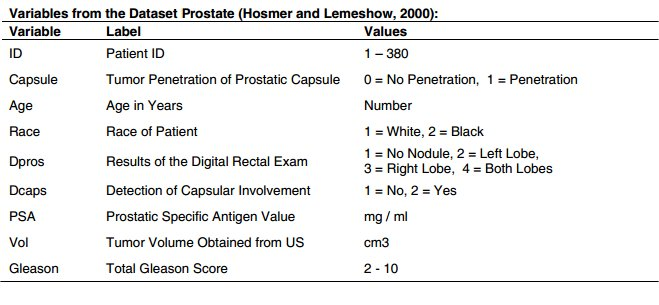
\includegraphics[scale=0.6]{images/LogWeek10C.jpg}\\
  \caption{Variables}
\end{figure}
\end{center}
\subsection{Kasser and Bruce Infarction Data Example}
We use a set of coronary data (Kasser and Bruce, 1969;
Kronmal and Tarter, 1974) to see if age, history of angina pectoris (ANGINA:
yes, no), history of high blood pressure (HIGHBP: yes, no), and functional class
(FUNCTION: none, minimal, moderate, and more than moderate) can be used to
predict the probability of past myocardial infarction (INFARCT: yes, no).


\end{document}